\documentclass[9pt,pdf,hyperref={unicode}]{beamer}
\beamertemplatenavigationsymbolsempty

\setbeamertemplate{blocks}[rounded=true, shadow=true]
\setbeamertemplate{footline}[page number]
\usepackage{multicol}

\usefonttheme{serif}

\usepackage[utf8]{inputenc}
\usepackage[english, russian]{babel}
\usepackage{amsmath,mathrsfs,mathtext}
\usepackage{graphicx, epsfig}
\usepackage{caption}
\usepackage{subfig}
\usepackage{amsmath, bm}

\usepackage{comment}

\usepackage{tabularx}

\usepackage{tikz}

\DeclareMathOperator*{\argmin}{arg\,min}
\DeclareMathOperator*{\argmax}{arg\,max}
\usepackage{array}
\newcolumntype{L}[1]{>{\raggedright\let\newline\\\arraybackslash\hspace{0pt}}m{#1}}
\newcolumntype{C}[1]{>{\centering\let\newline\\\arraybackslash\hspace{0pt}}m{#1}}
\newcolumntype{R}[1]{>{\raggedleft\let\newline\\\arraybackslash\hspace{0pt}}m{#1}}

%formulas
\newcommand{\calA}{\mathcal{A}}
\newcommand{\calAx}{\mathcal{A}_x}
\newcommand{\calAy}{\mathcal{A}_y}
\newcommand{\calAz}{\mathcal{A}_z}
\newcommand{\calW}{\mathcal{W}}
\newcommand{\calWx}{\mathcal{W}_x}
\newcommand{\calWy}{\mathcal{W}_y}
\newcommand{\calWz}{\mathcal{W}_z}
\newcommand{\calT}{\mathcal{T}}
\newcommand{\calTx}{\mathcal{T}_x}
\newcommand{\calTy}{\mathcal{T}_y}
\newcommand{\calS}{\mathcal{S}}
\newcommand{\calSx}{\mathcal{S}_x}
\newcommand{\calSy}{\mathcal{S}_y}
\newcommand{\calSt}{\mathcal{S}_t}
\makeatletter
\let\@@magyar@captionfix\relax
\makeatother

\usetheme{Warsaw}
\usecolortheme{sidebartab}
\definecolor{beamer@blendedblue}{RGB}{31,96,49}

\setbeamertemplate{enumerate items}[circle]

\setbeamersize{text margin left=1.5em, text margin right=1.5em}

\usepackage{ragged2e}

%----------------------------------------------------------------------------------------------------------
\title[Trajectory estimation and step detection]
{Trajectory estimation and step detection}
\author[Filippova A.\ V.]{\Large Filippova Anastasia Vladislavovna}
\institute[]{\large Moscow Institute of Physics and Technology (National Research University)\\
~\\

Сonsultant: Gadaev T.\\
Expert:    Strijov V.\\
}

\date{April 30, 2020}
%----------------------------------------------------------------------------------------------------------
\begin{document}
%----------------------------------------------------------------------------------------------------------
\begin{frame}
\titlepage
\end{frame}

%----------------------------------------------------------------------------------------------------------
\begin{frame}{Trajectory estimation and step detection}

\begin{block}{Purpose} 
Propose a new pipeline for indoor navigation with Inertial Measurement Unit (IMU) sensors.
\end{block}

\begin{block}{Motivation} 
\begin{itemize}
    \item Indoor trajectory estimation
    \item Measure activity level
\end{itemize}{}
\end{block}

\begin{block}{Method}
\begin{itemize}
    \item Combine step detection and trajectory estimation
    \item Use instant velocities
    \item Use attention mechanism for instant velocities
\end{itemize}{}
\end{block}

\end{frame}
%----------------------------------------------------------------------------------------------------------

\begin{frame}{Problem statement}
Find the superposition of functions $F_{\text{tr}}$, which transforms sensors data to trajectory estimation and $F_{\text{st}}$ - to step labels.
    \begin{block}{Data}
        \begin{enumerate}
        \item $\calA \in \mathbb{R}^{3\times T}$ - accelerometer readings 
        \item $\calW \in \mathbb{R}^{3\times T}$ - gyroscope readings
        \item $\mathcal{S} \in \{0,1\}^2$ - steps labels
        \end{enumerate}
    \end{block}

    \begin{block}{Minimization of loss function}
        \begin{equation}
            \label{eq:general_ps}
            \argmin\limits_{F_{\text{tr}}, F_{\text{st}}}\mathcal{L}\left(\left(F_{\text{tr}}\left(\calA, \calW\right), \calT\right),(F_{\text{st}}\left(\calA, \calW\right), \calS\right)
        \end{equation}{}
    \end{block}
    \textbf{Combined loss function:}
    \begin{block}{Loss function} 
       \begin{equation*}
            \label{nohyper}
             \mathcal{L}(\hat{\textbf{y}_t}, \textbf{y}_t) =  \|\hat{\textbf{v}_x} - \textbf{v}_t\|_2^2 - w(s_r \log p_r + s_l \log p_l) , y_t = \left( v_x^t , v_y^t, s_r^t, s_l^t\right)
        \end{equation*}
    \end{block}
\begin{enumerate}
\item $s_r^t, s_l^t$ - steps labels for right and left legs at timestamp $t$.
\item $v_x^t, v_y^t$ - velocities on timestamp $t$.
\item $p_r^t, p_l^t$ - predicted probability of step.
\end{enumerate}
\end{frame}
\begin{frame}{Metrics}
\begin{block}{\textbf{RMSE}}
Absolute trajectory error (\textbf{RMSE}) defined as the root mean square error between predicted and ground truth trajectories:
\begin{equation}
    \mathcal{L_{\text{tr}}}(\hat{\calT}, \calT) = (\frac{1}{N}\sum_{i=1}^N ((\hat{t_x}_i - {t_x}_i)^2 + (\hat{t_y}_i - {t_y}_i)^2))^{^1/_2}
\end{equation}
\end{block}
\begin{block}{\textbf{MIE}}
Mean integral distance (\textbf{MIE}) between predicted and ground truth trajectories:
\begin{equation}
    \mathcal{D_{\text{tr}}}(\hat{\calT}, \calT) = \frac{
    \sum_{i=1}^N ((\hat{t_x}_i - {t_x}_i)^2 + (\hat{t_y}_i - {t_y}_i)^2)^{^1/_2}  (({t_x}_i - {t_x}_{i-1})^2 + ({t_y}_i - {t_y}_{i-1})^2)^{^1/_2}}{\sum_{i=1}^N (({t_x}_i - {t_x}_{i-1})^2 +({t_y}_i - {t_y}_{i-1})^2)^{^1/_2}}
\end{equation}
\end{block}
\end{frame}
\begin{frame}{Metrics}
\begin{block}{\textbf{GAP}}
Distance between the first and the last points (\textbf{GAP}):
\begin{equation}
    \label{eq:metric_gap}
    \mathcal{G_{\text{tr}}}\left(\hat{\calT}\right) =  \left(\left(\hat{t_x}_1 - \hat{t_x}_{N}\right)^2 + \left(\hat{t_y}_1 - \hat{t_y}_{N}\right)^2\right)^{^1/_2}
\end{equation}{}
\end{block}
\begin{block}{\textbf{RTE}}
Relative trajectory error defined as the average RMSE over a fixed time interval~--- $w$, if the sequence is shorter than $w$ we compute the positional error and scale it proportionally:
\begin{equation}
    \label{eq:metric_rte}
    \mathcal{R_{\text{tr}}}(w, \hat{\calT}, \calT) \approx \frac{1}{\lfloor N/w\rfloor}\sum_{i=1}^{\lfloor N/w\rfloor}(\frac{1}{w}\sum_{i=1}^w ((\hat{t_x}_{kw + i} - {t_x}_{kw + i})^2 + (\hat{t_y}_{kw + i} - {t_y}_{kw + i})^2))^{^1/_2}
\end{equation}{}
\end{block}
\end{frame}
%----------------------------------------------------------------------------------------------------------
\begin{frame}[shrink=5]{Baseline model}

\center{ResNet-18 without the last layer stacked with two LSTM layers}
\begin{figure}
\begin{minipage}[!h]{1\linewidth}
\center{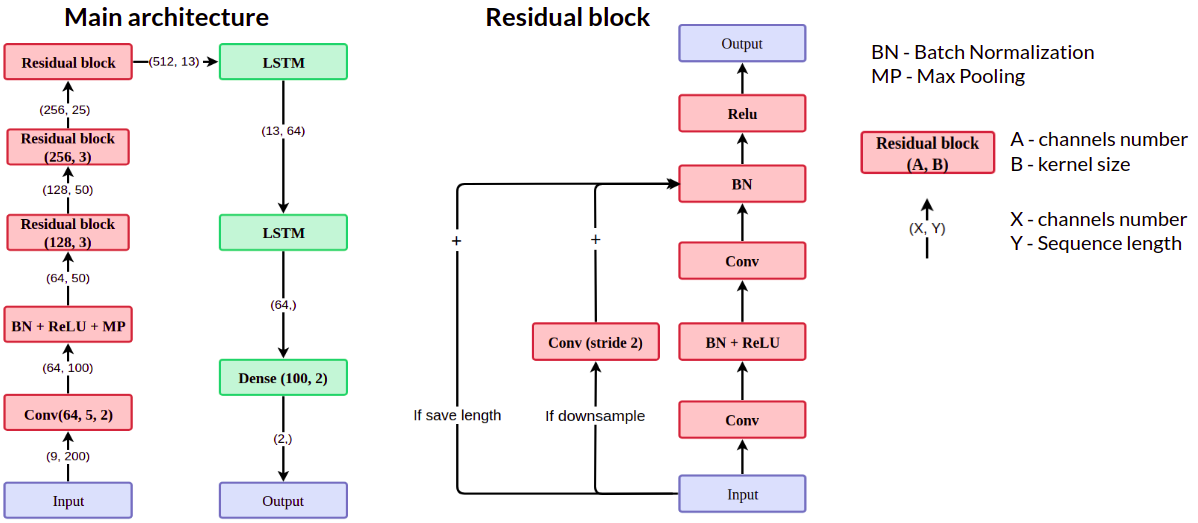
\includegraphics[width=1\linewidth]{final.png}\\Baseline model}
\end{minipage}

\end{figure}




\end{frame}
%----------------------------------------------------------------------------------------------------------
\begin{frame}[shrink=5]{ResNetLSTM with step detection}

\begin{figure}
\begin{minipage}[!h]{1.01\linewidth}
\center{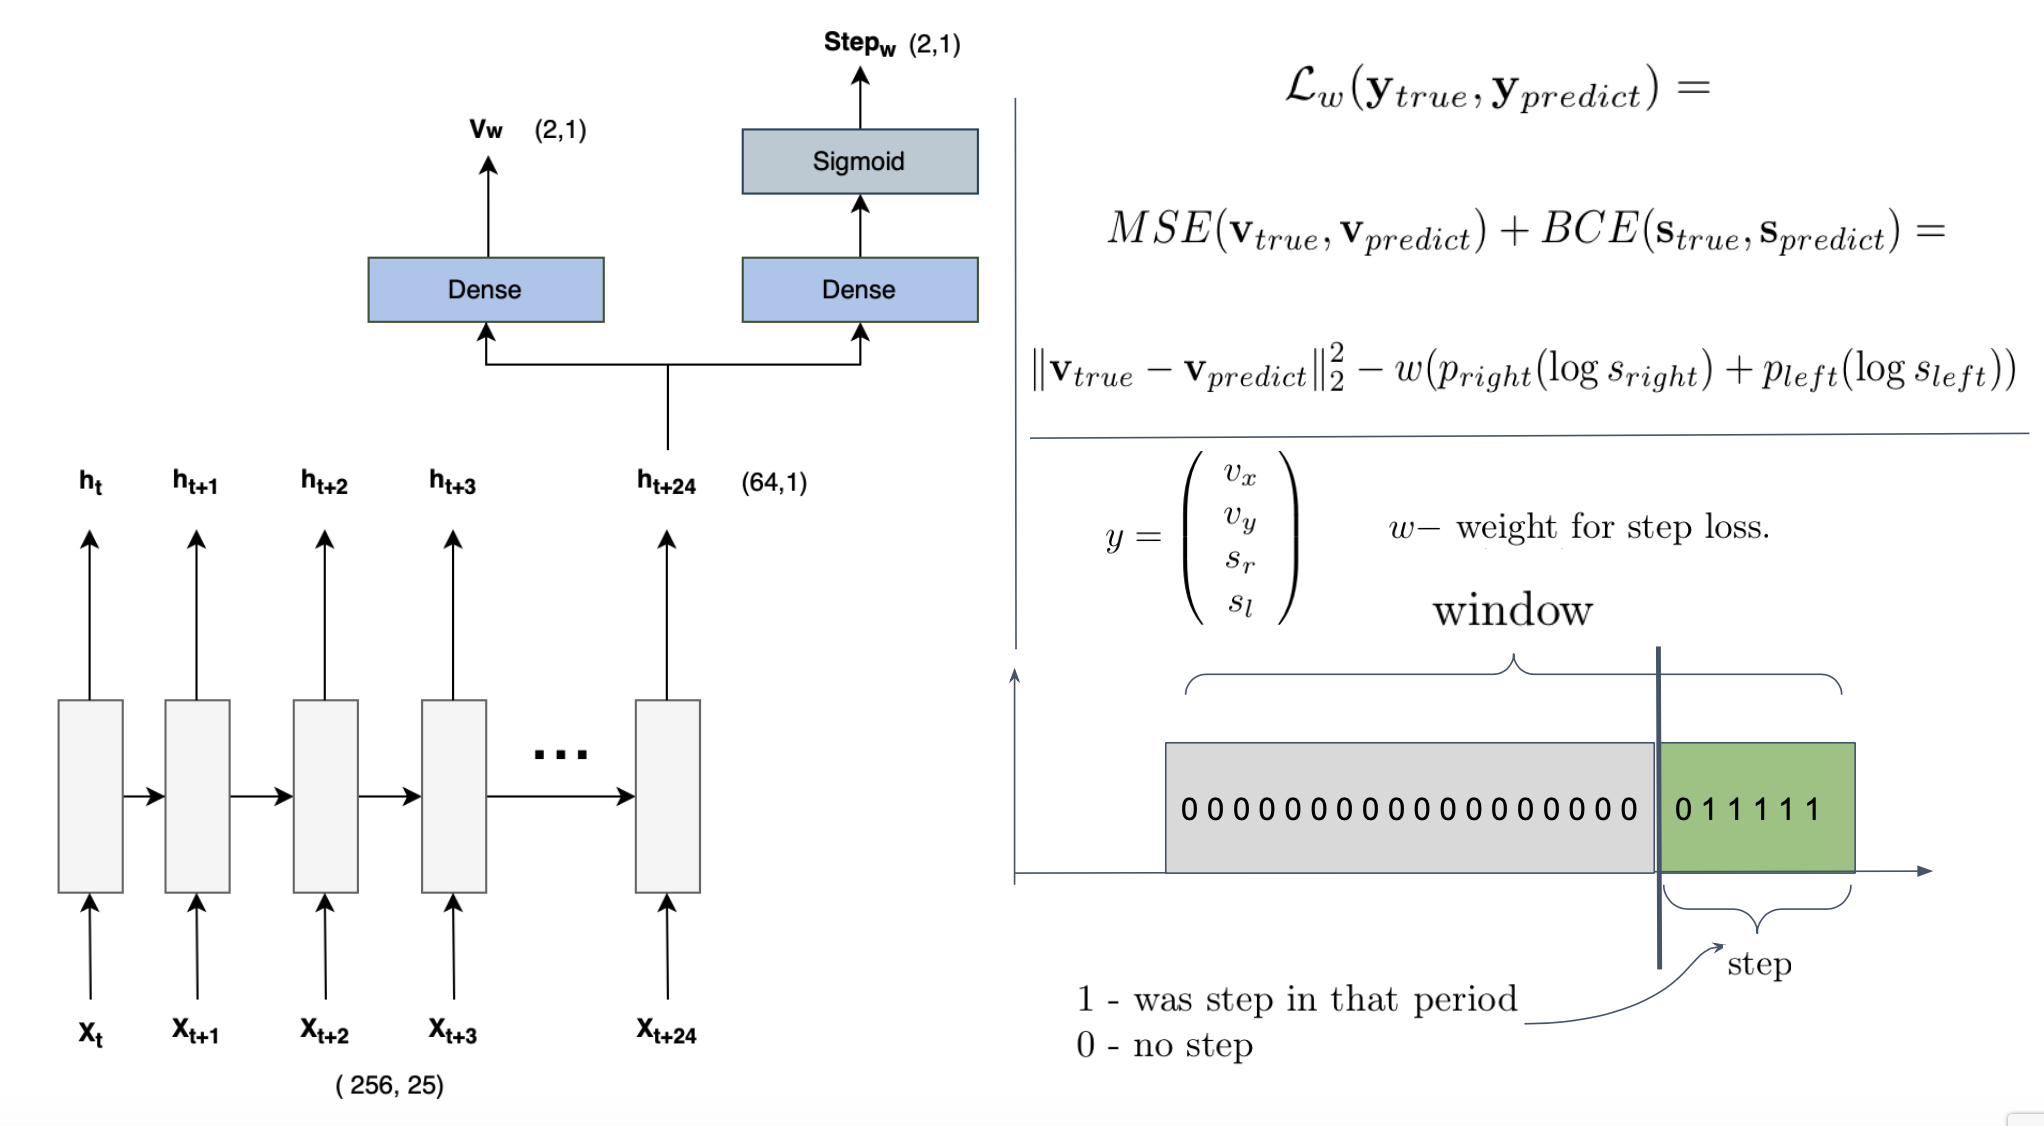
\includegraphics[width=1\linewidth]{First.png}}
\end{minipage}

\end{figure}




\end{frame}
%----------------------------------------------------------------------------------------------------------

\begin{frame}[shrink=5]{Results ResNetLSTM with step detection}

\begin{figure}
\begin{minipage}[!h]{1\linewidth}
\center{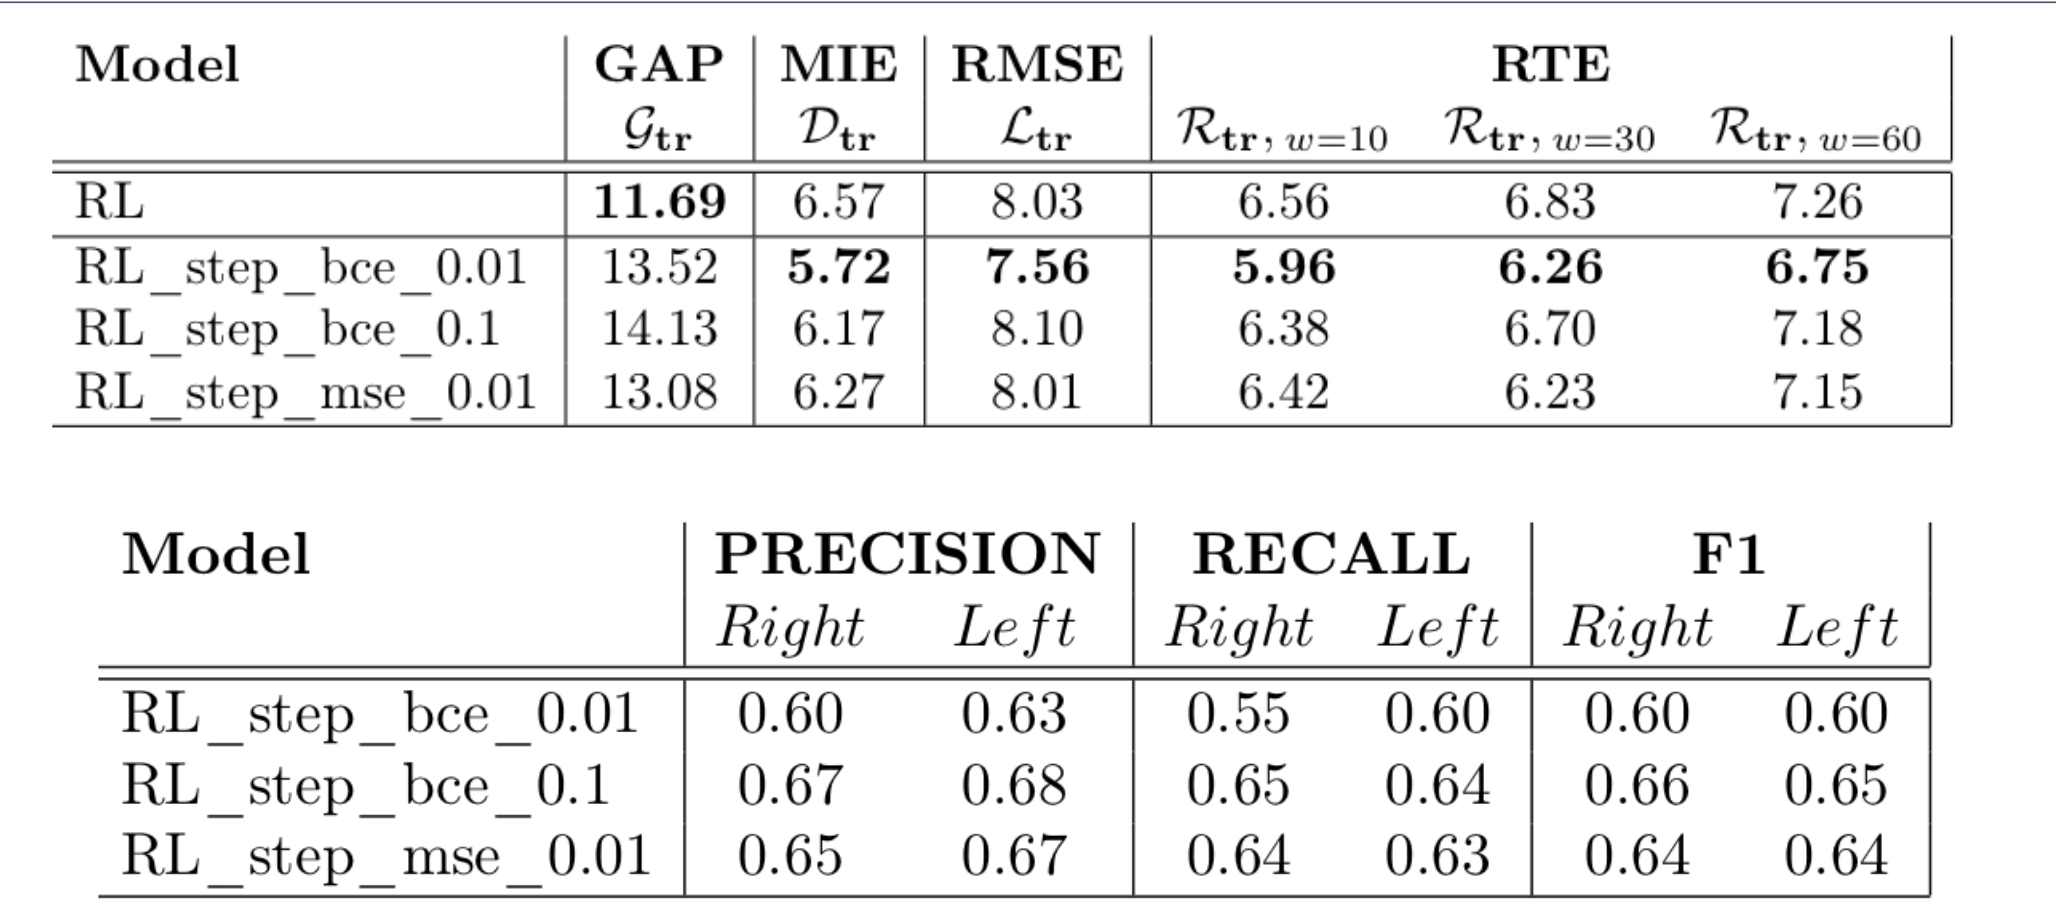
\includegraphics[width=1\linewidth]{First results.png}\\ResNetLSTM and step detection results}
\end{minipage}

\end{figure}





\end{frame}
%----------------------------------------------------------------------------------------------------------
\begin{frame}[shrink=5]{Instant velocities}

\begin{figure}
\begin{minipage}[!h]{1\linewidth}
\center{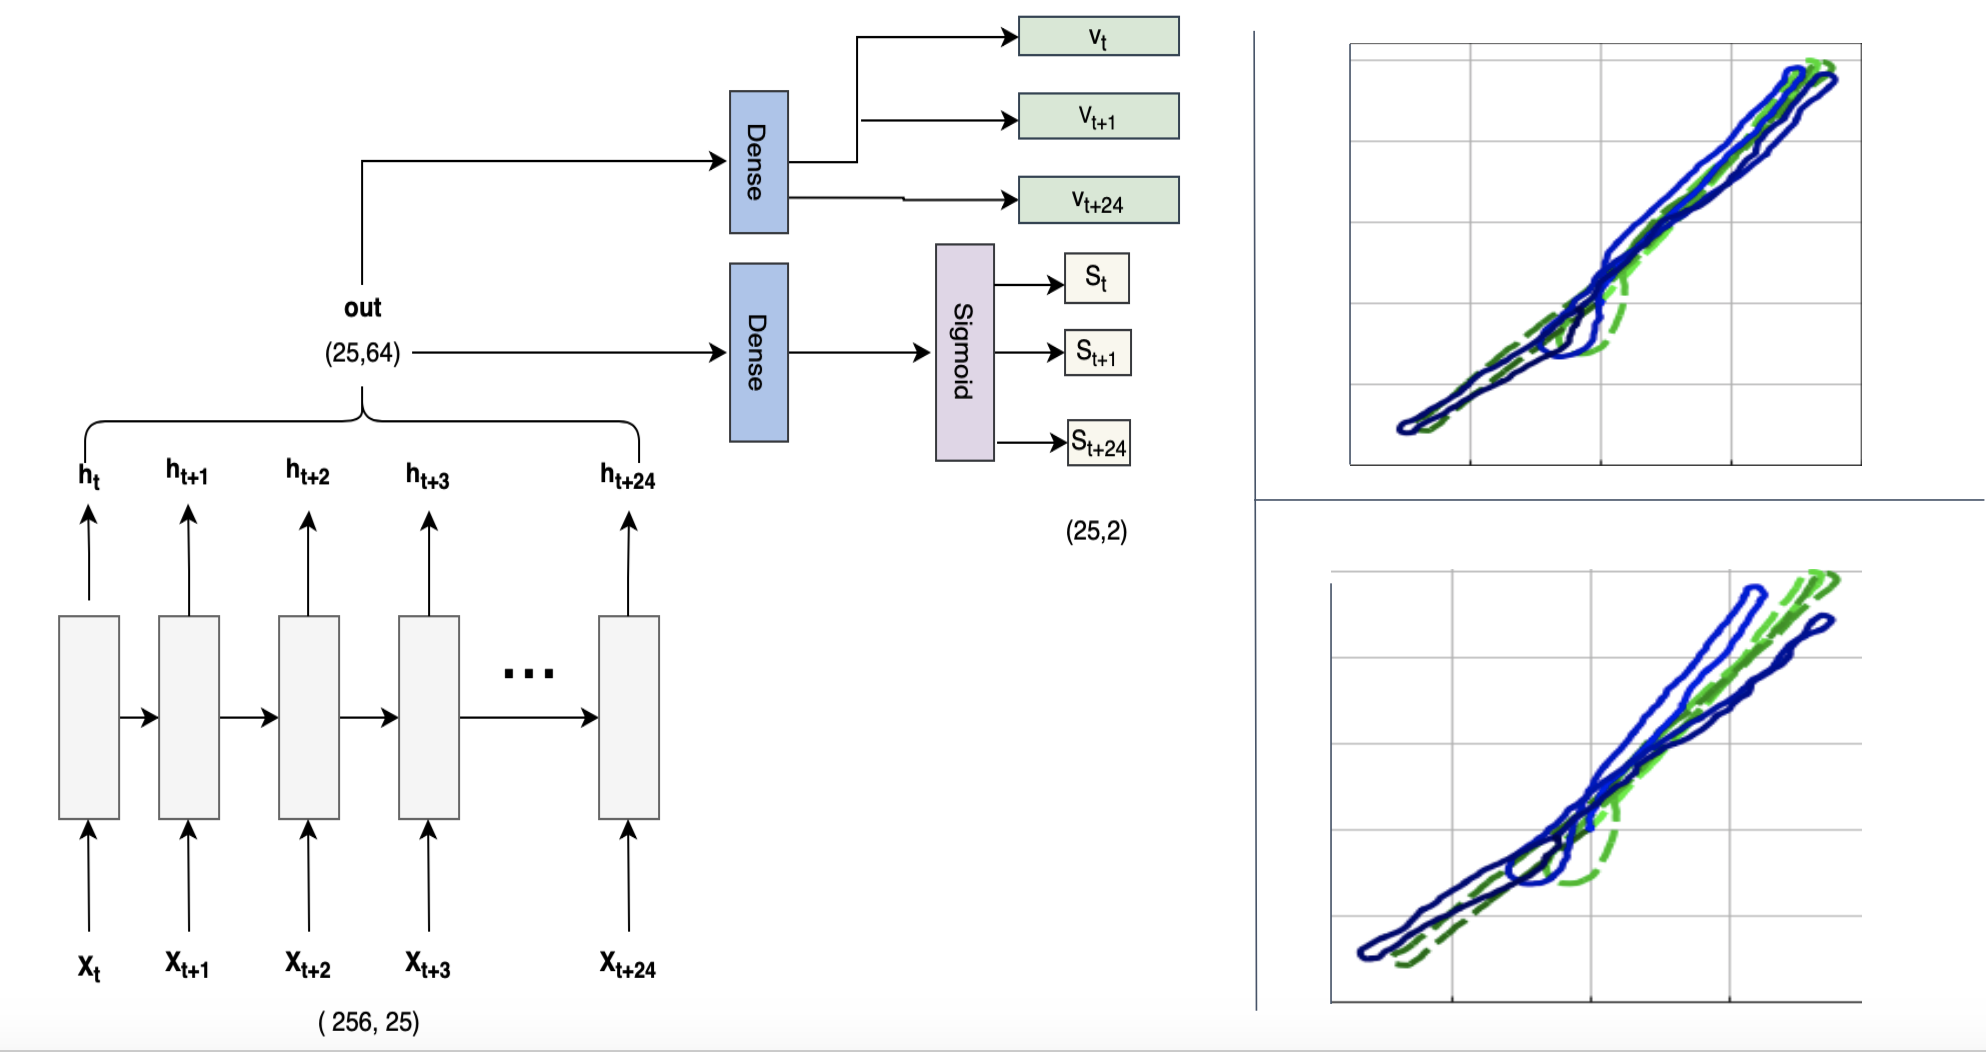
\includegraphics[width=1.1\linewidth]{Second.png}\\ Architecture and comparison}
\end{minipage}

\end{figure}





\end{frame}
%----------------------------------------------------------------------------------------------------------
\begin{frame}[shrink=5]{Results ResNetLSTM with instant velocities}
\begin{figure}
\begin{minipage}[!h]{1\linewidth}
\center{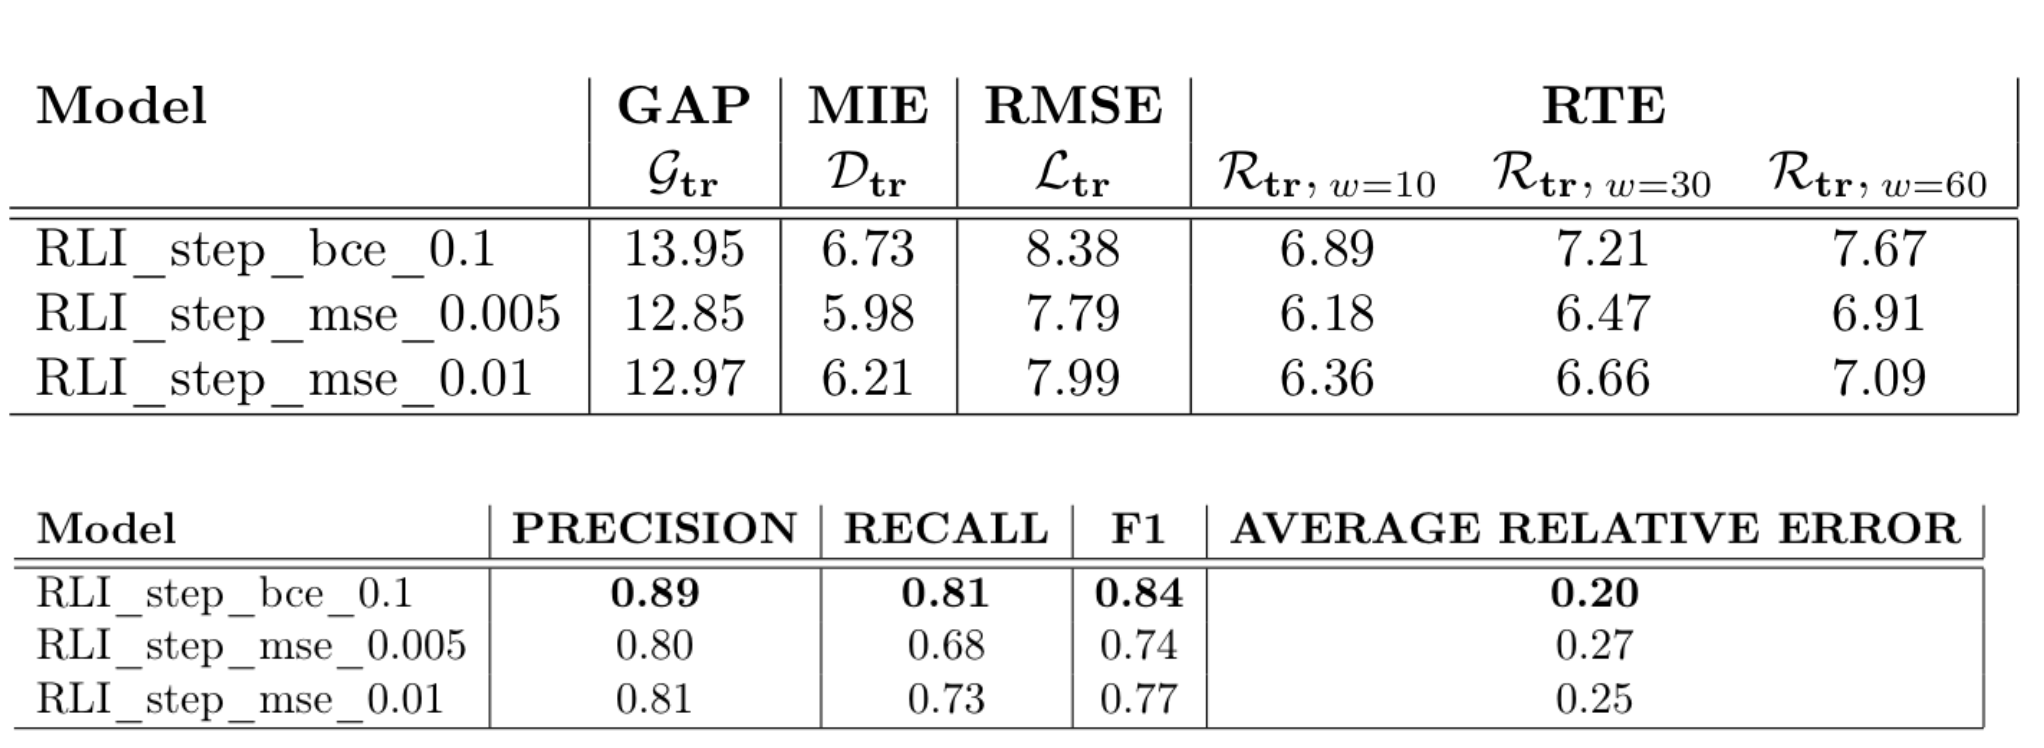
\includegraphics[width=1.01\linewidth]{Second results.png}\\ResNetLSTM Instant velocity and step detection results}
\end{minipage}

\end{figure}





\end{frame}
%----------------------------------------------------------------------------------------------------------
\begin{frame}[shrink=5]{Attention mechanism}
\begin{figure}
\begin{minipage}[!h]{1\linewidth}
\center{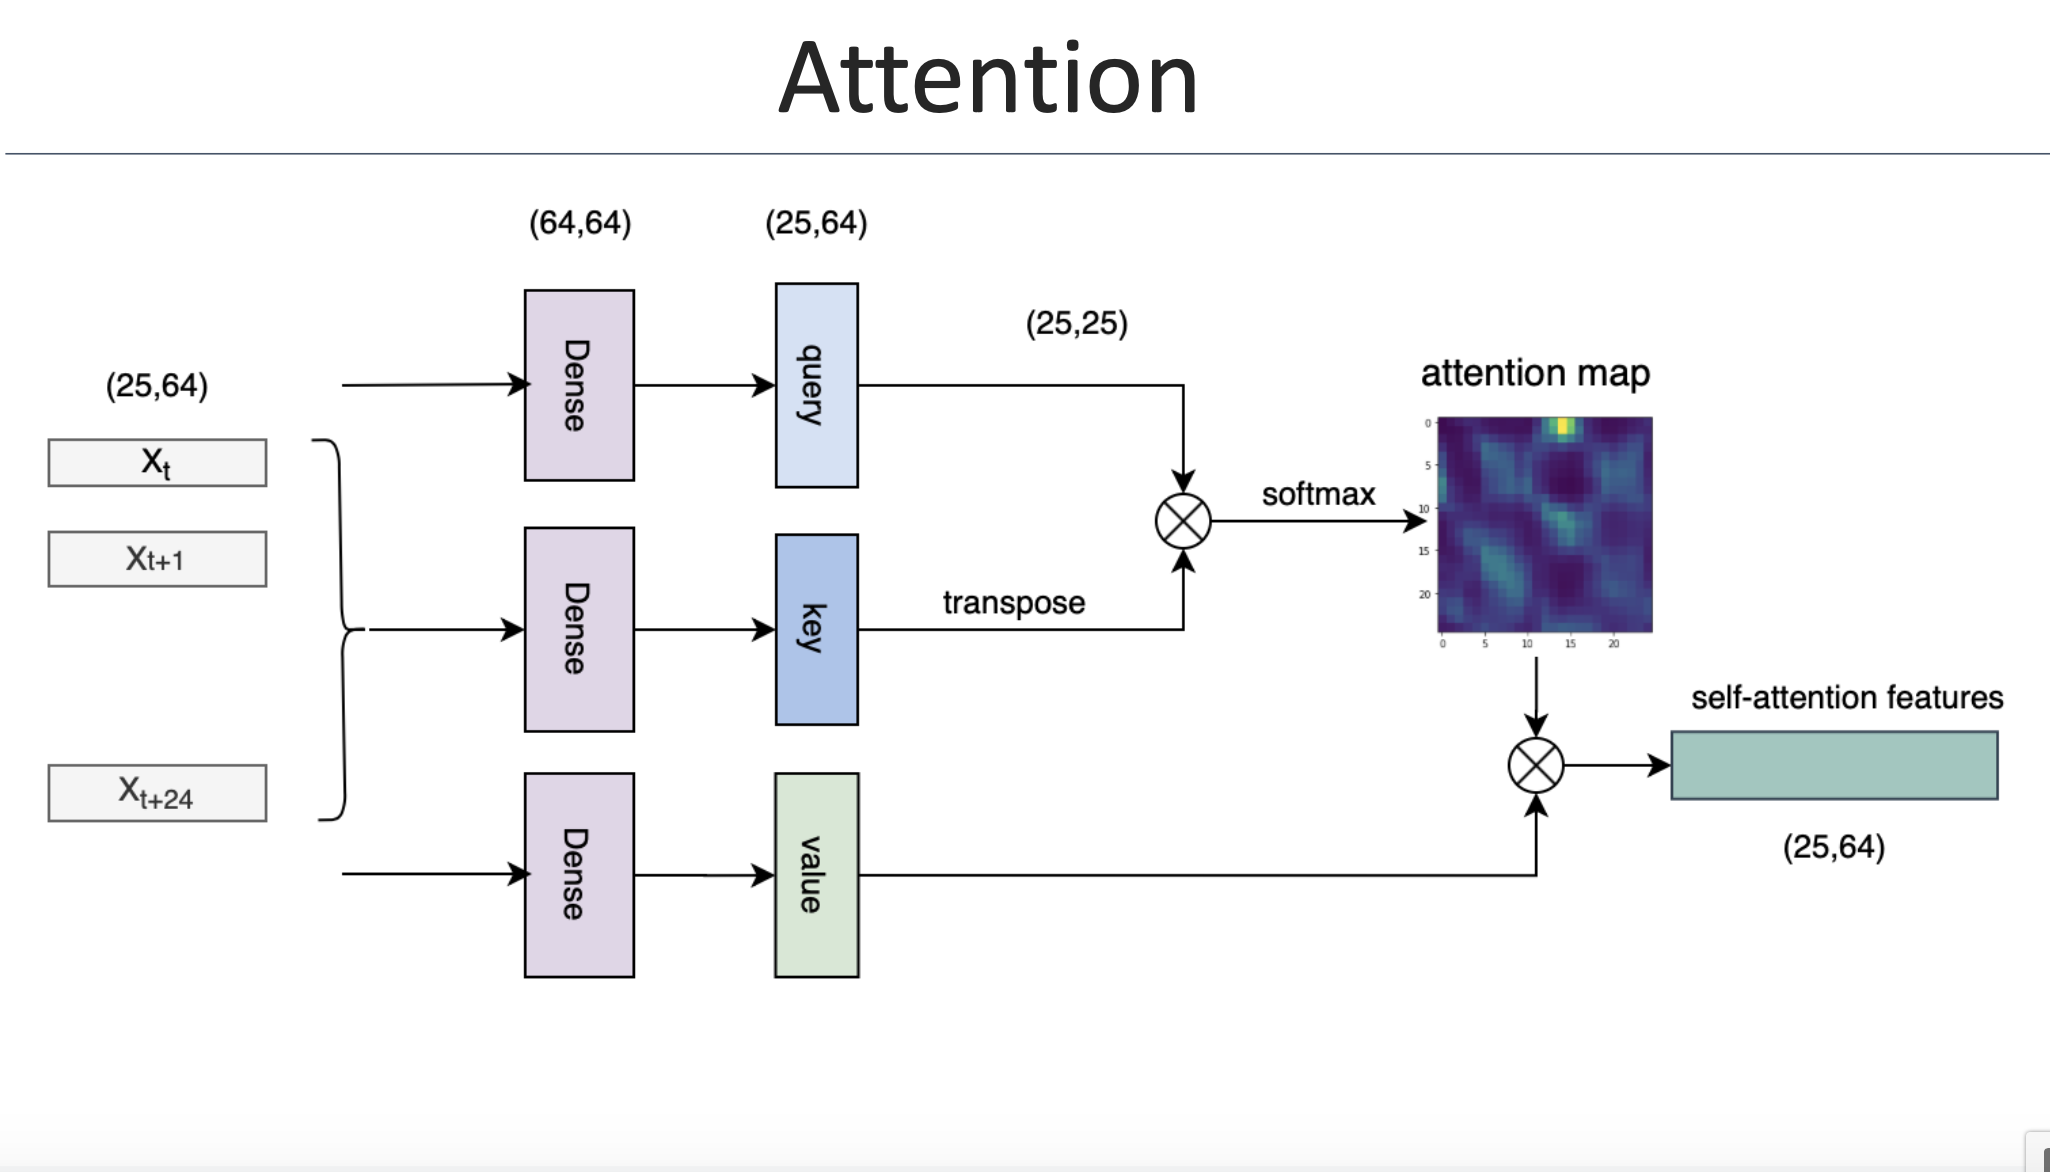
\includegraphics[width=1.01\linewidth]{Third.png}\\Attention layer}
\end{minipage}

\end{figure}





\end{frame}
%----------------------------------------------------------------------------------------------------------

\begin{frame}[shrink=5]{Attention maps}
\begin{figure}
\begin{minipage}[!h]{1\linewidth}
\center{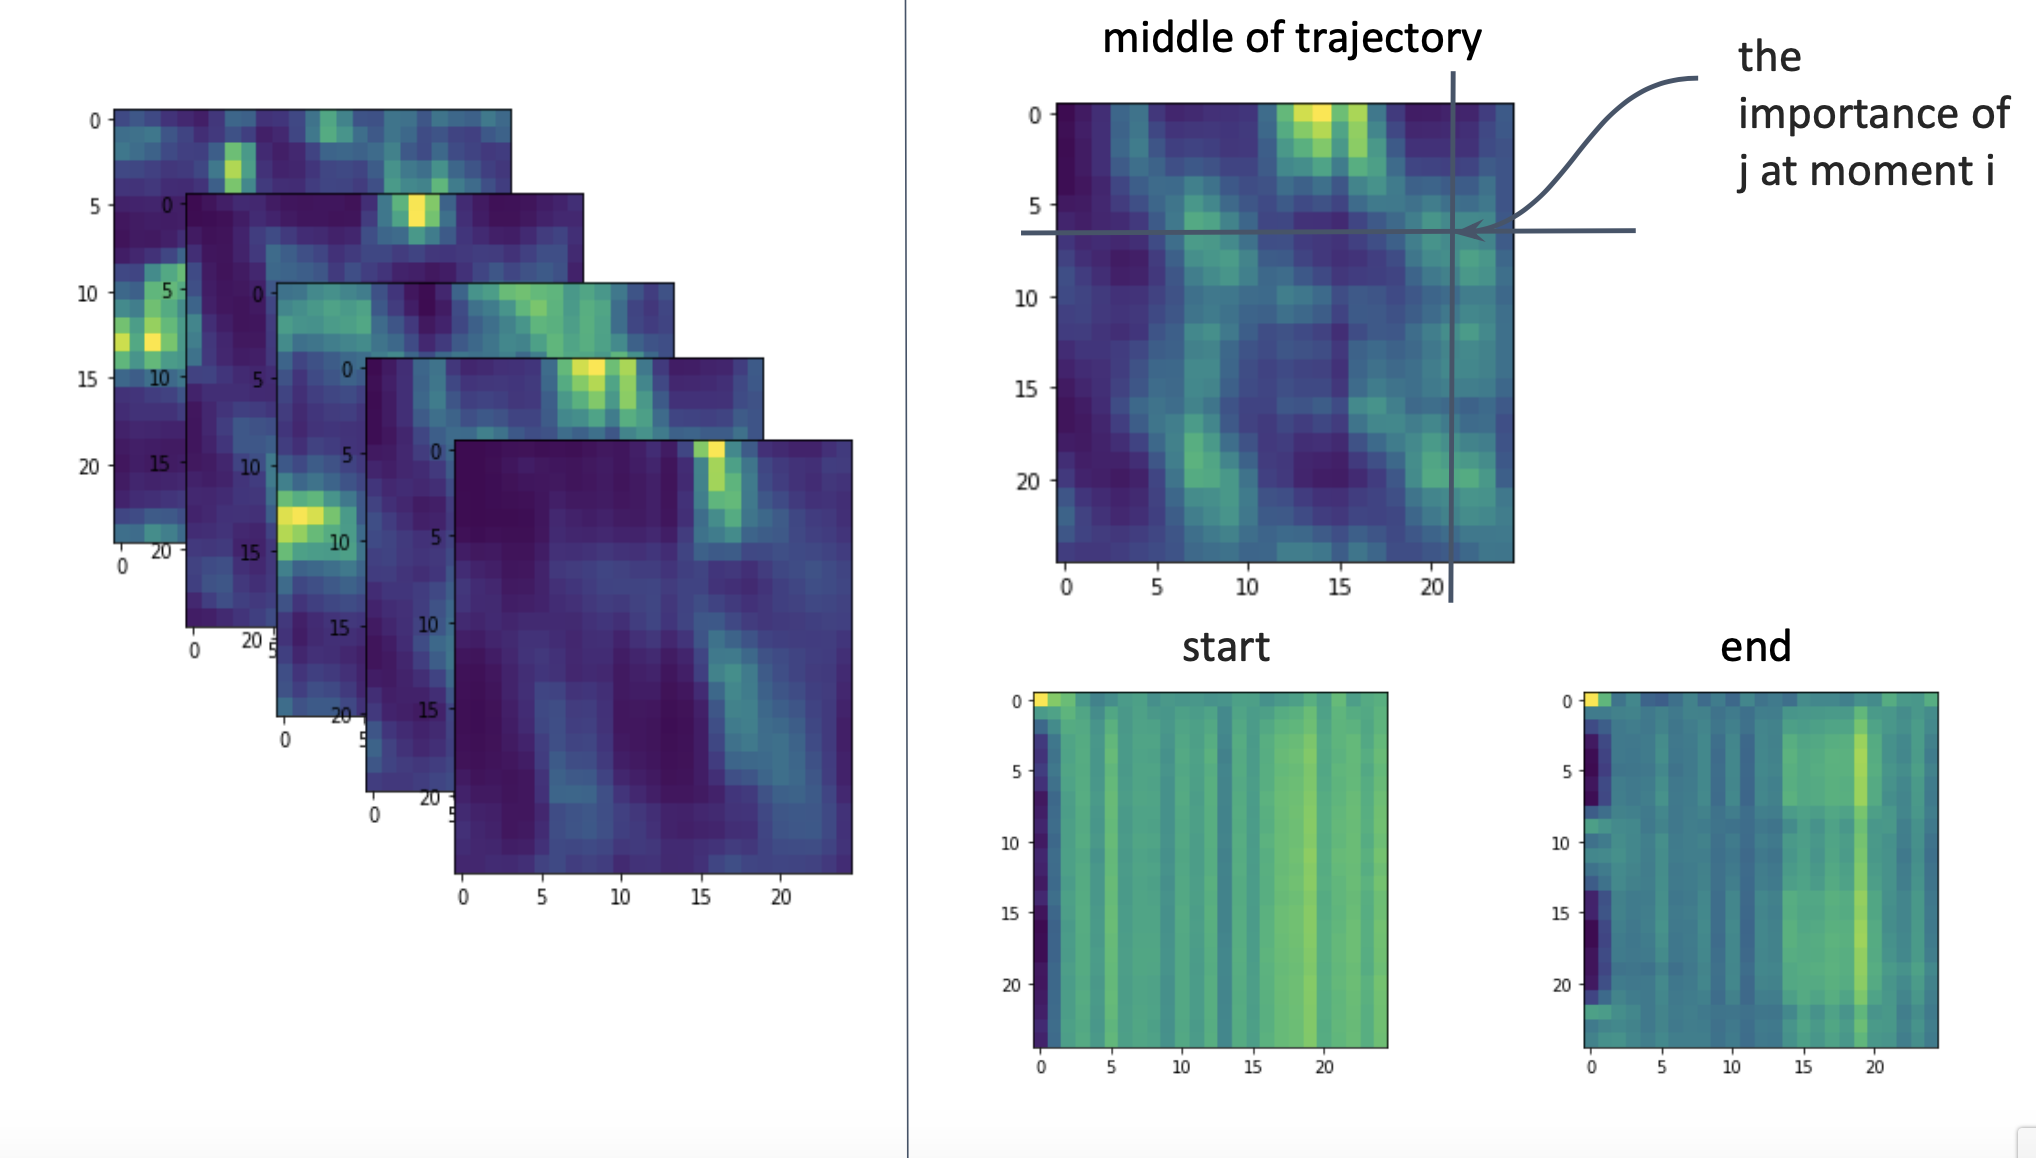
\includegraphics[width=1.01\linewidth]{Attention maps.png}}
\end{minipage}

\end{figure}





\end{frame}

\begin{frame}[shrink=5]{Results attention}
\begin{figure}
\begin{minipage}[!h]{1\linewidth}
\center{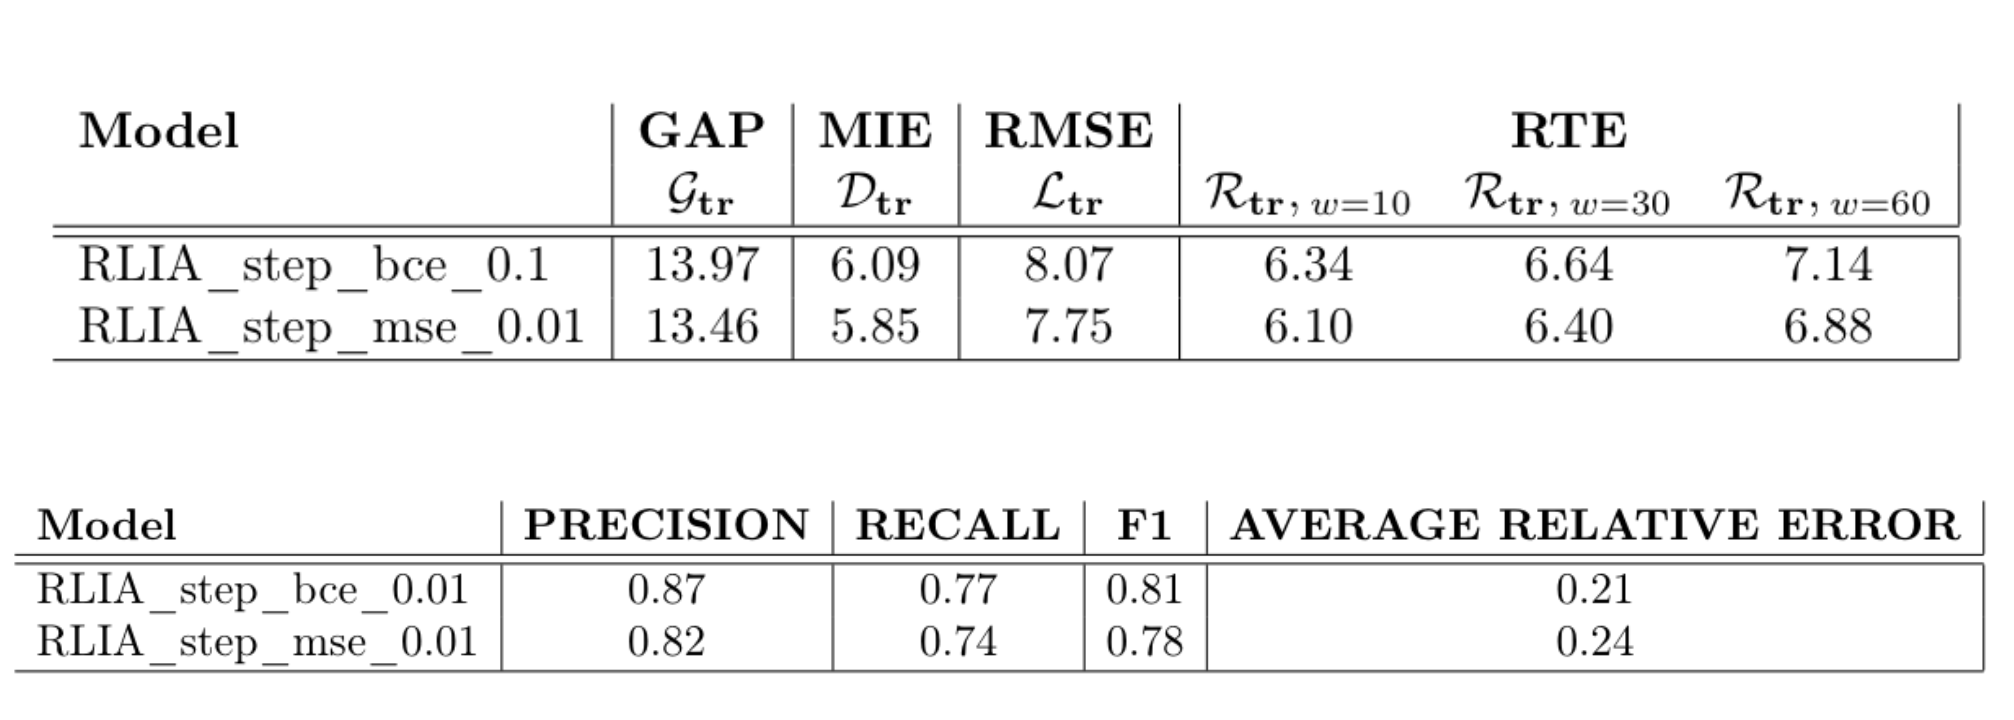
\includegraphics[width=1.01\linewidth]{Third results.png}\\ResNetLSTM with self-attention and step detection results}
\end{minipage}

\end{figure}





\end{frame}

\begin{frame}{Conclusion and future work}
\justifying

	\begin{enumerate}
	\justifying
	\item The quality of the proposed models is much better than quality of baseline approach.
	\item The average relative error for step detection is less then $0.27$.
    \item Attention gives good quality and can be test on other datasets.
	\end{enumerate}
	


\end{frame}


\end{document} 
